\chapter{Introduction}
\section{Problem Statement}
The dataset is related to red variants of the Portuguese "Vinho Verde" wine.The dataset describes the amount of various chemicals present in wine and their effect on it's quality. The datasets can be viewed as classification or regression tasks. The classes are ordered and not balanced (e.g. there are much more normal wines than excellent or poor ones).Task is to predict the quality of wine using the given data.

A simple yet challenging project, to anticipate the quality of wine.

The complexity arises due to the fact that the dataset has fewer samples, \& is highly imbalanced.

\textbf{Data Source} : \href{https://archive.ics.uci.edu/ml/datasets/wine+quality}{https://archive.ics.uci.edu/ml/datasets/wine+quality}

\section{About Dataset}
The dataset contains the following columns:
\begin{enumerate}
    \item fixed acidity
    \item volatile acidity
    \item citric acid
    \item residual sugar
    \item chlorides
    \item free sulfur dioxide
    \item total sulfur dioxide
    \item density
    \item pH
    \item sulphates
    \item alcohol
    \item quality (Targe Variable) : ranges from 0 to 10
\end{enumerate}

The data information is as follow:
\begin{figure}[H]
    \centering
    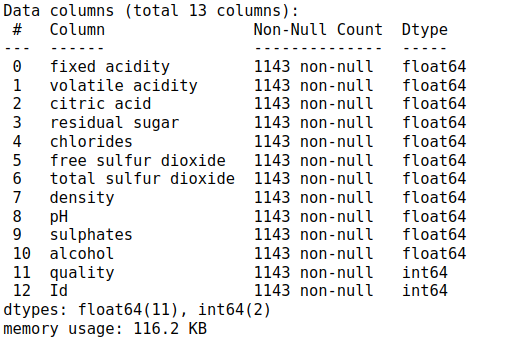
\includegraphics[scale = 0.7]{data_info.png}
    \caption{Data Information}
    \label{fig:Data Information}
\end{figure}





\section{Dataset Statistics}
The count plot of the whole dataset on the basis of quality of wine is shown below.

\begin{figure}[H]
    \centering
    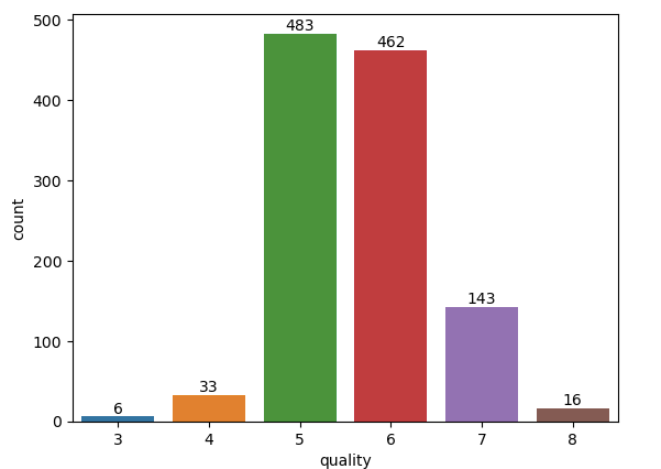
\includegraphics[scale = 0.7]{data_statistics/whole_dataset_countplot.png}
    \caption{Quality Count plot}
    \label{fig:Quality Count plot}
\end{figure}

We can see from above countplot, that the data is highly imbalanced and quality of wine(0, 1, 2, 9, 10) are not present in the dataset.

In order to deal with this imbalanced, at first we are going to merge the quality labels (3 and 4) and (7 and 8) as shown below.


\begin{figure}[H]
    \centering
    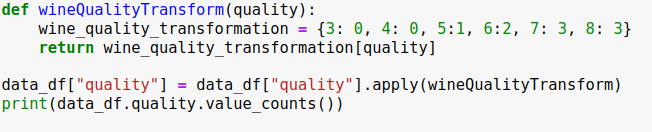
\includegraphics[scale = 0.7]{data_statistics/wineQualityTransformCode.png}
    \caption{Code for transformation of quality attribute}
    \label{fig:Code for transformation of quality attribute}
\end{figure}

The resulting count plot is as shown below:
\begin{figure}[H]
    \centering
    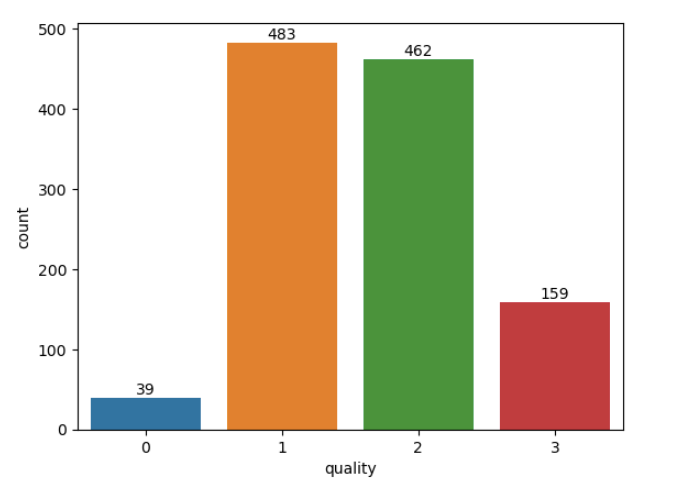
\includegraphics[scale = 0.7]{data_statistics/transformed_whole_dataset_countplot.png}
    \caption{Quality Count plot after transformation}
    \label{fig:Quality Count plot after transformation}
\end{figure}

\subsection{Train, validation and test dataset}
We are going to use 80\%, and 20\% of the dataset as training, validation and test data. The countplot are as shown below:

\begin{figure}[H]
    \centering
    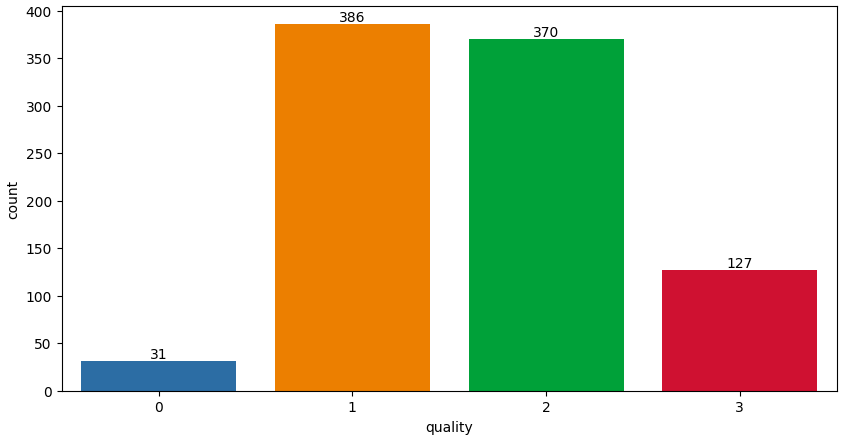
\includegraphics[scale = 0.5]{data_statistics/train_dataset.png}
    \caption{Train Quality Count plot after transformation}
    \label{fig:Train Quality Count plot after transformation}
\end{figure}


\begin{figure}[H]
    \centering
    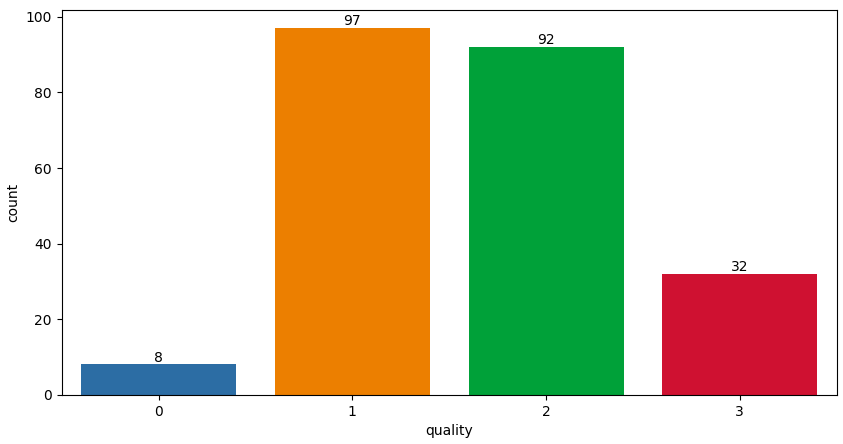
\includegraphics[scale = 0.5]{data_statistics/test_dataset.png}
    \caption{Test Quality Count plot after transformation}
    \label{fig:Test Quality Count plot after transformation}
\end{figure}

\section{Literature Review}
Several studies have been conducted to model wine preferences by data mining from physicochemical properties. For example, Cortez et al. (2009) used a dataset of 1599 red wines to develop a model that predicts wine quality based on 11 physicochemical properties. They used decision tree, support vector machine, and artificial neural network algorithms to model wine quality, and found that the artificial neural network algorithm had the highest accuracy. Similarly, Araújo and Juliano (2011) used a dataset of 649 Portuguese white wines to develop a model that predicts wine quality based on physicochemical properties. They used decision tree, logistic regression, and artificial neural network algorithms to model wine quality, and found that the artificial neural network algorithm had the highest accuracy.

Other studies have focused on modeling wine preferences based on specific physicochemical properties. For example, Medina et al. (2017) used a dataset of 167 Spanish red wines to develop a model that predicts wine preference based on phenolic compounds. They used partial least squares regression and support vector machine algorithms to model wine preference, and found that the support vector machine algorithm had the highest accuracy. Similarly, Li et al. (2016) used a dataset of 80 Chinese red wines to develop a model that predicts wine preference based on aroma compounds. They used a fuzzy comprehensive evaluation method to model wine preference, and found that the method had a high accuracy.

Several studies have also investigated the relationship between physicochemical properties and wine sensory attributes. For example, Escudero et al. (2017) used a dataset of 100 Spanish red wines to study the relationship between physicochemical properties and wine sensory attributes. They found that several physicochemical properties, such as pH, alcohol content, and total phenolic content, were significantly correlated with wine sensory attributes, such as color intensity, aroma intensity, and astringency. Similarly, Jolliffe et al. (2016) used a dataset of 301 Australian white wines to study the relationship between physicochemical properties and wine sensory attributes. They found that several physicochemical properties, such as pH, titratable acidity, and residual sugar, were significantly correlated with wine sensory attributes, such as fruity, floral, and herbaceous aromas.

Data mining techniques have been widely used to model wine preferences based on physicochemical properties. Several studies have shown that these techniques can accurately predict wine quality and preference based on specific physicochemical properties, such as phenolic compounds and aroma compounds. Additionally, studies have found significant correlations between physicochemical properties and wine sensory attributes, suggesting that physicochemical properties play an important role in determining wine quality and consumer preferences. These findings have important implications for the wine industry, as they can be used to improve wine quality and tailor wines to specific consumer preferences.


\section{Outcome}
We expect the output to be the list of probabilites of belonging to a class[0, 1, 2 or 3]. Among these, the class with higher probability is out predicted class. 

For the application of wine quality classification, we have developed a web app using django for backend and react for frontend whose screenshot is given below.

\begin{figure}[H]
    \centering
    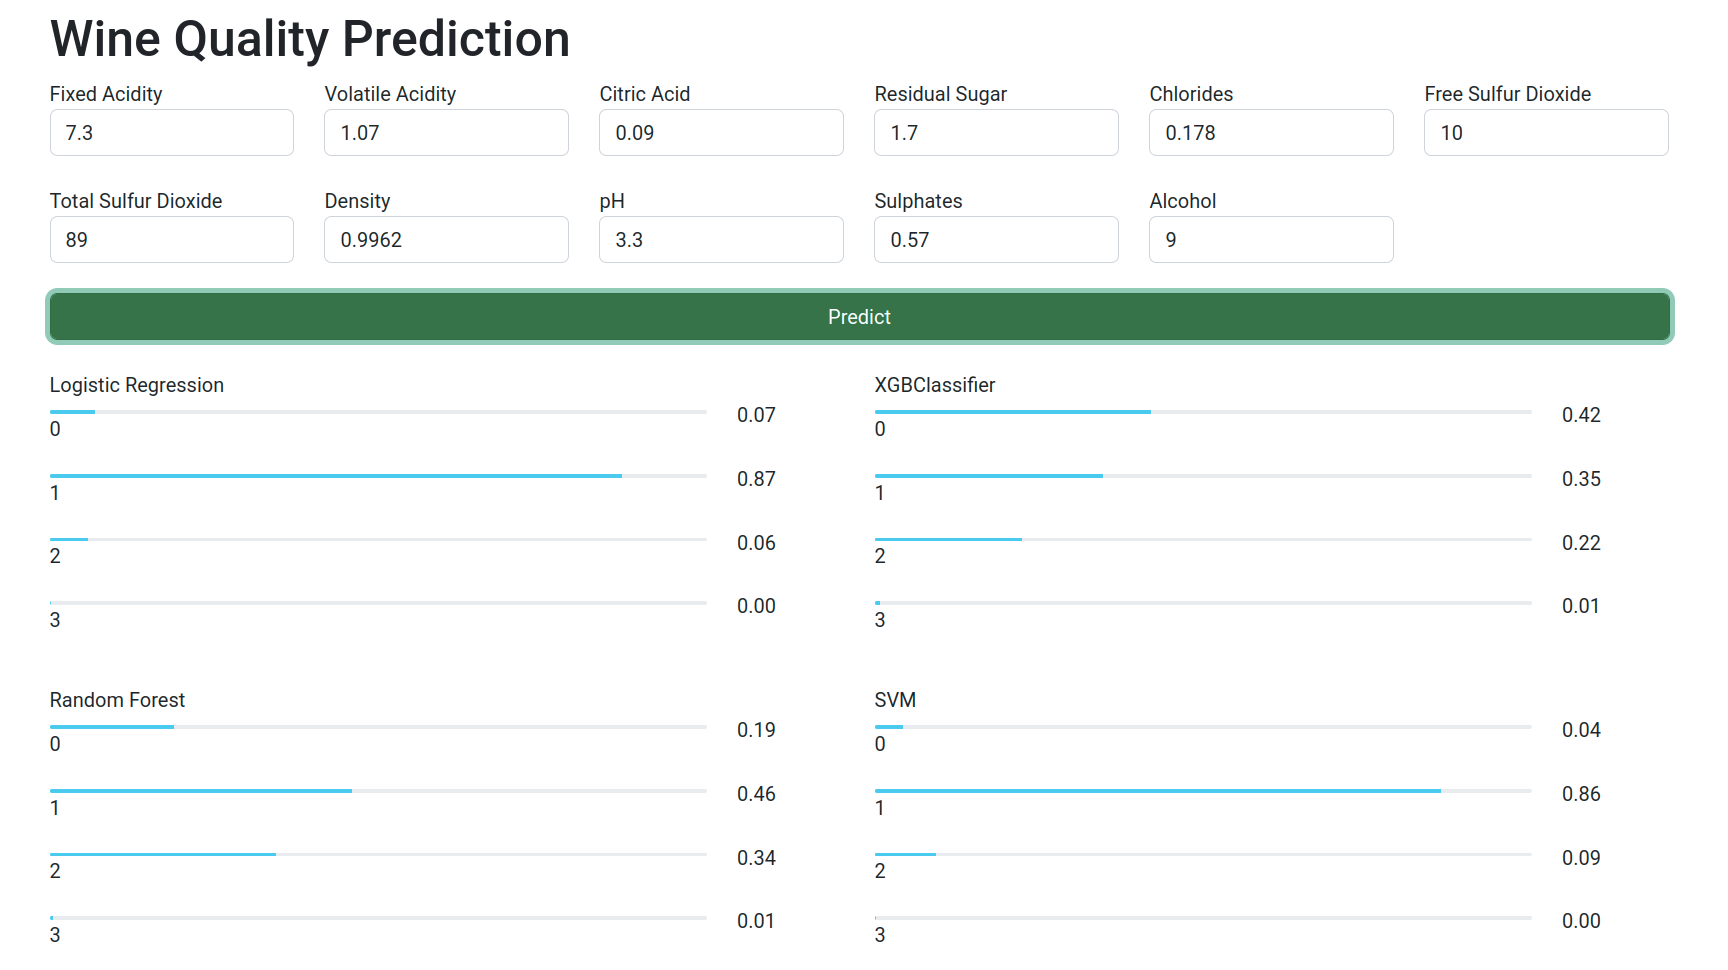
\includegraphics[scale = 0.27]{frontend.png}
    \caption{Frontend}
\end{figure}

